\documentclass[a4paper, titlepage]{article}
\usepackage[round, sort, numbers]{natbib}
\usepackage[utf8]{inputenc}
\usepackage{amsfonts, amsmath, amssymb, amsthm}
\usepackage{color}
\usepackage{framed}
\usepackage{listings}
\usepackage{mathtools}
\usepackage{paralist}
\usepackage{parskip}
\usepackage{subfig}
\usepackage{tikz}
\usepackage{titlesec}
%\usepackage{ulem}

\numberwithin{figure}{section}
\numberwithin{table}{section}

\usetikzlibrary{arrows, automata, backgrounds, petri, positioning}
\tikzstyle{place}=[circle, draw=blue!50, fill=blue!20, thick]
\tikzstyle{transition}=[rectangle, draw=black!50, fill=black!20, thick, minimum width=5.5mm, minimum height=5.5mm]

% define new commands for sets and tuple
\newcommand{\setof}[1]{\ensuremath{\left \{ #1 \right \}}}
\newcommand{\tuple}[1]{\ensuremath{\left \langle #1 \right \rangle }}
\newcommand{\card}[1]{\ensuremath{\left \vert #1 \right \vert }}

\definecolor{lstbg}{rgb}{1,1,0.9}
\lstset{basicstyle=\ttfamily, numberstyle=\tiny, breaklines=true, backgroundcolor=\color{lstbg}, frame=single}
\lstset{language=C}

\makeatletter
\newcommand\deadline[1]{\def\@deadline{#1}}
\newcommand\objective[1]{\def\@objective{#1}}
\newcommand{\makecustomtitle}{%
	\begin{center}
		\huge\@title \\
		[1ex]\small Dimitri Racordon, le \@date
	\end{center}
	\begin{framed}\@deadline\end{framed}
	\begin{framed}\@objective\end{framed}
}
\makeatother

\begin{document}

\title{Outils formels de Modélisation \\ 2\textsuperscript{ème} Travail personnel}
\author{Dimitri Racordon}
\date{13.10.17}

\deadline{
\textbf{Date de rendu}: Jeudi 26.10.17 à 23h55 \\

  Comme leur nom l'indique, ces travaux sont \emph{personnels}.
  La copie est strictement interdite, et toutes similitudes entre deux rendus
  seront santionnées par la note de 0.
  Tout dépassement de la date et heure de rendu sera lourdement pénalisée.
  Date et heure de rendu sont toujours données en heure locale de Genève.
  Tout commit sur votre dépôt publié après la date de rendu sera ignoré.

  Seule la branche \texttt{master} de votre dépôt sera prise en compte
  lors de la correction.

  Votre code doit être compilable en Swift 4.0, avec un compilateur officiel.
  La note the 1 vous sera attribuée si votre code ne peut être compilé.
}

\objective{
  Dans ce TP, vous allez modéliser un problème classique de concurrence
  à l’aide des réseaux de Petri et en étudierez les propriétés.
}

\makecustomtitle

\section{Les fumeurs de cigare}

Dans cet exerice, nous allons modéliser le problème des fumeurs de cigarettes.
Ce problème, énoncé par Suhas Patil \cite{patil:1971}, se présente de la manière suivante:

Pour fabriquer et fumer une cigarette, trois ingrédients sont nécessaires:
\begin{inparaenum}[\itshape 1\upshape)]
  \item du papier à rouler;
  \item du tabac;
  \item une allumette.
\end{inparaenum}
Un certain nombre de fumeurs en chaîne sont assis autour d'une table ronde,
disposant chacun d'un ingrédient différent,
en quantité infinie.
De plus, un \emph{arbitre} est également assis à la table
et dispose quant à lui de tous les ingrédients, en quantités infinies.

L'arbtitre choisit aléatoirement deux des trois ingrédients et les pose sur la table.
Le fumeur disposant de celui manquant saisit alors les ingrédients sur la table
et les utilise pour fabriquer et fumer une cigarette.

L'arbitre ne fait rien dès lors que quelque chose est posé sur la table,
et attend que cette dernière soit à nouveau vide.
Un fumeur ne se saisit pas des ingrédients manquants tant qu'il fume déjà une cigarette.
Ces restrictions mises à part, chaque acteur répète inlassablement son processus respectif.

La figure \ref{fig:smokers} représente une possible modélisation du problème des fumeurs de cigare,
pour 4 fumeurs.

\begin{figure}[ht]
  \centering
  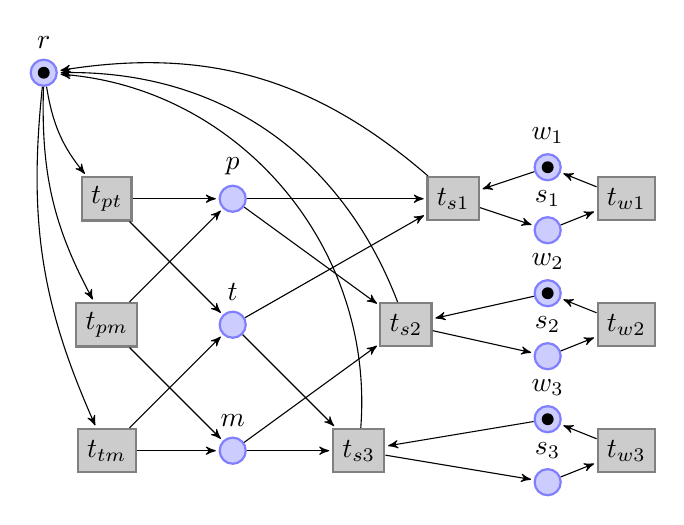
\begin{tikzpicture}[node distance=16mm,>=stealth',bend angle=15,auto]
    % Ingredients.
    \node[place] (p) [label=90:$p$] {};
    \node[place] (t) [below of=p, label=90:$t$] {};
    \node[place] (m) [below of=t, label=90:$m$] {};

    % Referee.
    \node[place, tokens=1] (r) [above of=p, xshift=-24mm, label=90:$r$] {};
    \node[transition] (tpt) [left of=p] {$t_{pt}$}
      edge[pre, bend left] (r)
      edge[post] (p)
      edge[post] (t);
    \node[transition] (tpm) [left of=t] {$t_{pm}$}
      edge[pre, bend left] (r)
      edge[post] (p)
      edge[post] (m);
    \node[transition] (ttm) [left of=m] {$t_{tm}$}
      edge[pre, bend left] (r)
      edge[post] (t)
      edge[post] (m);

    % 1st smoker.
    \node[place, tokens=1] (w1) [right of=p, xshift=24mm, yshift=4mm, label=90:$w_1$] {};
    \node[place] (s1) [right of=p, xshift=24mm, yshift=-4mm, label=90:$s_1$] {};
    \node[transition] (ts1) [right of=p, xshift=12mm] {$t_{s1}$}
      edge[pre]  (p)
      edge[pre]  (t)
      edge[pre]  (w1)
      edge[post] (s1)
      edge[post, bend right=25] (r);
    \node[transition] (tw1) [right of=p, xshift=34mm] {$t_{w1}$}
      edge[pre]  (s1)
      edge[post] (w1);

    % 2nd smoker.
    \node[place, tokens=1] (w2) [right of=t, xshift=24mm, yshift=4mm, label=90:$w_2$] {};
    \node[place] (s2) [right of=t, xshift=24mm, yshift=-4mm, label=90:$s_2$] {};
    \node[transition] (ts2) [right of=t, xshift=6mm] {$t_{s2}$}
      edge[pre]  (p)
      edge[pre]  (m)
      edge[pre]  (w2)
      edge[post] (s2)
      edge[post, bend right=35] (r);
    \node[transition] (tw2) [right of=t, xshift=34mm] {$t_{w2}$}
      edge[pre]  (s2)
      edge[post] (w2);

    % 3rd smoker.
    \node[place, tokens=1] (w3) [right of=m, xshift=24mm, yshift=4mm, label=90:$w_3$] {};
    \node[place] (s3) [right of=m, xshift=24mm, yshift=-4mm, label=90:$s_3$] {};
    \node[transition] (ts3) [right of=m] {$t_{s3}$}
      edge[pre]  (t)
      edge[pre]  (m)
      edge[pre]  (w3)
      edge[post] (s3)
      edge[post, bend right=45] (r);
    \node[transition] (tw3) [right of=m, xshift=34mm] {$t_{w3}$}
      edge[pre]  (s3)
      edge[post] (w3);
  \end{tikzpicture}

  \caption{Problème des fumeurs de cigare}
  \label{fig:smokers}
\end{figure}

\section{Mise en place du TP}

Forkez le dépôt https://github.com/cui-unige/outils-formels-modelisation.
Vous travaillerez sur votre propre version du dépôt,
et effectuerez tous vos commit sur ce dépôt-ci.

Le projet pour ce TP se trouve dans le répertoire \texttt{tp-02}.

\section{Modélisation du problème}

Encodez le réseau de la figure \ref{fig:smokers} à l'aide de la libraire PetriKit.
\textbf{Veillez à respecter le nom des places et des transitions.}
Par exemple, la transition nommée $t_{s2}$ doit porter le nom \texttt{ts2} dans votre code.
Les tests associés à ce travail ne passeront pas si vous ne respectez pas cette consigne!

\section{Analyse du modèle}

La méthode \texttt{PTNet.markingGraph(from:)}
(dans le fichier \texttt{PTNet+Extensions.swift})
est supposée retourner le graphe de marquage d'un réseau Pétri,
d'après un marquage initial donné.

Ecrivez l'implémentation de cette fonction,
puis utilisez-la pour générer le graphe de marquage de votre réseau
et répondre aux questions suivantes:

\begin{enumerate}
  \item Combien d'états différents votre réseau peut-il avoir?
  \item Est-il possible que deux fumeurs différents fument en même temps.
  \item Est-il possible d'avoir deux fois le même ingrédient sur la table.
\end{enumerate}

\begin{thebibliography}{9}

\bibitem{patil:1971}
  S. Patil,
  \emph{Limitations and Capabilities of Dijkstra's Semaphore Primitives for Coordination Among Processes}.
  Project MAC,
  Computational Structures Group Memo 57,
  1971.

\end{thebibliography}

\end{document}
